\begin{figure}[p]
  \centering
  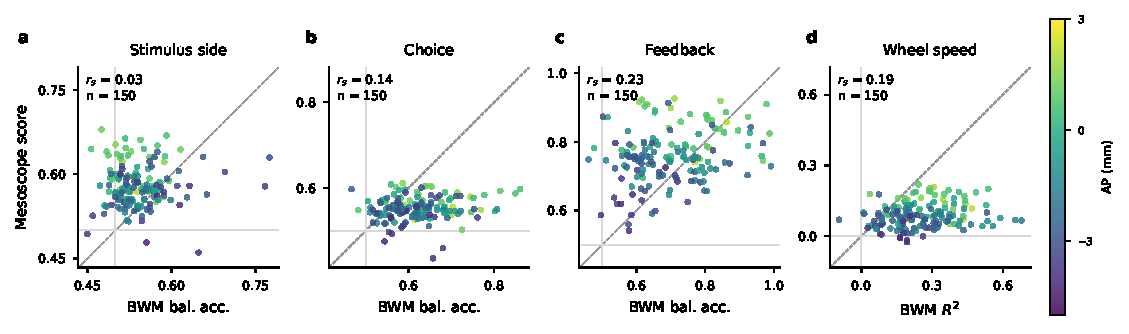
\includegraphics[width=7.00in,height=0.78\textheight,keepaspectratio]{figures/fig7_decoding_all_scatter/dorsal_decoding_all_scatter_panels.pdf}
  \caption{Decoding per spatial bin, BWM Neuropixels (x) vs mesoscope (y), decoded from all neurons of the session in the bin. Each point is one hexagonal bin (0.4\,mm, hemispheres folded) with at least one session of each modality contributing $\geq$10 neurons; its value is the score averaged across those sessions (same values as the decoding maps). Colour: AP position of the bin. Dashed line: identity; grey lines: chance (0.5 balanced accuracy, 0 for $R^2$). The $p$-values ignore spatial autocorrelation between neighbouring bins and are therefore optimistic. With all neurons, mesoscope bins hold far more neurons than BWM bins, which inflates the mesoscope scores. \textbf{a} Stimulus side (Spearman $r_s = 0.03$, $p = 0.7$, 150 bins). \textbf{b} Choice (Spearman $r_s = 0.14$, $p = 0.092$, 150 bins). \textbf{c} Feedback (Spearman $r_s = 0.23$, $p = 0.005$, 150 bins). \textbf{d} Wheel speed, cross-validated $R^2$ (Spearman $r_s = 0.19$, $p = 0.017$, 150 bins).}
  \label{fig:fig7_decoding_all_scatter}
\end{figure}
